\documentclass[aspectratio=169]{beamer}
% \documentclass[aspectratio=169,handout]{beamer}

\usetheme[titleformat=regular%
,numbering=fraction% use slide numbers
]{metropolis}
\metroset{%
  progressbar=foot,%
  %background=dark,
  block=fill
}
\only<handout>{\metroset{sectionpage=none}}
\only<handout>{\usecolortheme{dove}}
\usepackage{appendixnumberbeamer} % separate appendix
\usepackage[citestyle=authortitle,sorting=none]{biblatex}
\setbeamerfont{footnote}{size=\tiny}
\addbibresource{mae.bib}

% multimedia in beamer presentations
\usepackage{multimedia}

% adding some better facilities to latex such as proper booleans
\usepackage{etoolbox}

% Unicode math symbols for XeLaTeX
\usepackage{mathrsfs}

% standard math packages
\usepackage{amssymb}
\usepackage{amsthm}
\usepackage{amsmath}
\usepackage{amstext}
\usepackage{mathabx}
\usepackage{stmaryrd}
% math tools for amsmath
\usepackage{mathtools}

\usepackage{proof}

\usepackage{listings}
\usepackage{xcolor}

% subfigures, subfloats
\usepackage{subcaption}

% for multiinclude
\usepackage{xmpmulti}

% tikz & friends

\usepackage{galois}
\usepackage{tikz}
\usetikzlibrary{fit,calc,shapes,arrows.meta,patterns,backgrounds}
\usetikzlibrary{decorations.pathmorphing}
\usetikzlibrary{cd}
\usepackage[beamer]{hf-tikz}

\newcommand{\tikzmark}[1]{%
  \tikz[overlay,remember picture,baseline] \node [anchor=base] (#1) {};}

\newenvironment{tightcenter}{%
  \setlength\topsep{0pt}
  \setlength\parskip{0pt}
  \begin{center}
}{%
  \end{center}
}

% new colors
\definecolor{lightblue}{RGB}{217,220,253}
\definecolor{lightred}{RGB}{251,216,218}

\DeclareMathOperator{\pw}{\mathcal{P}} % powerset
\newcommand{\fset}[1]{\mathsf{#1}}
\newcommand{\nats}{\mathbb{N}}
\newcommand{\zahlen}{\mathbb{Z}}
\newcommand{\bools}{\mathbb{B}}
\newcommand{\Set}[1]{\left\{#1\right\}}
\newcommand{\true}{\kw{true}}
\newcommand{\false}{\kw{false}}
\newcommand{\sidenote}[1]{\hfill\quad \textsf{#1}}

\newcommand{\disunion}{+}

% named set
\newcommand{\ns}[1]{\mathit{#1}}
% function
\newcommand{\fn}[1]{\mathrm{#1}}
% "vector of"
\newcommand{\vo}[1]{\overrightarrow{#1}}
% "set of"
\newcommand{\setOf}[1]{\overline{#1}}
% syntactic tag
\newcommand{\sTag}[2]{\textsf{\textbf{#1}}\,#2}
% keyword
\newcommand{\kw}[1]{\texttt{#1}}
% usual suspects
\newcommand{\State}{\ns{State}}
\newcommand{\Value}{\ns{Value}}
\newcommand{\Stmt}{\ns{Stmt}}
\newcommand{\Env}{\ns{Env}}
\newcommand{\Store}{\ns{Store}}
\newcommand{\Kont}{\ns{Kont}}
% syntactic domains
\newcommand{\Exp}{\ns{Exp}}
\newcommand{\Var}{\ns{Var}}
\newcommand{\Addr}{\ns{Addr}}
% put a value to a pointer
\newcommand{\update}{\leftarrow}

% ebnf
\newcommand{\eDEF}{\,::=\;}
\newcommand{\eOR}{\;\vert\;}

\newcommand{\widen}{\nabla}

% \newcommand{\|}{\,\vert\,}

\newcommand{\todo}[1]{\iftoggle{TODO}{\textcolor{red}{TODO: #1}}{}}
% ceiling and floor symbols
\DeclarePairedDelimiter\ceil{\lceil}{\rceil}
\DeclarePairedDelimiter\floor{\lfloor}{\rfloor}

% big O notation
\DeclareMathOperator{\bigO}{O}

% fixed points
\DeclareMathOperator{\lfp}{lfp}

% print both years for bibliography
\renewbibmacro*{cite:labelyear+extrayear}{%
\iffieldundef{labelyear}
{}
{\printtext[bibhyperref]{%
\iffieldundef{origyear}{}{\printfield{origyear}\addslash}%   <--- added
\printfield{labelyear}%
\printfield{extrayear}}}}

\renewbibmacro*{date+extrayear}{%
\iffieldundef{year}
{}
{\printtext[parens]{%
\iffieldundef{origyear}{}{\printfield{origyear}\addslash}%  <--- added
\printdateextra}}}

% overlay an image
\def\Put(#1,#2)#3{\leavevmode\makebox(0,0){\put(#1,#2){#3}}}

% text over symbols nicely, requires amsmath for overset
\newcommand\textoverop[2]{\mathrel{\overset{\makebox[0pt]{\mbox{\normalfont\tiny\sffamily #1}}}{#2}}}

% special arrows
\newcommand\monarrow{\textoverop{mon}{\rightarrow}}

% theorems
\newtheorem{thm}{Theorem}
\newtheorem{eg}{Example}

\newcommand{\abscolor}[1]{\textcolor{mLightBrown}{#1}}
\newcommand{\concolor}[1]{\textcolor{mLightGreen}{#1}}
\newcommand{\abst}[1]{#1^{\#}}

\newcommand{\step}{\rightsquigarrow}

% listings setup
\lstset{basicstyle=\tiny\ttfamily,columns=fixed}

%%% Local Variables:
%%% mode: latex
%%% TeX-master: "main"
%%% TeX-engine: xetex
%%% End:


\only<handout>{
  \pgfpagesuselayout{4 on 1}[letterpaper,border shrink=5mm,landscape]
}

\newtoggle{notes}
%\only<beamer>{\toggletrue{notes}}

% add notes:
\iftoggle{notes}{
  \makeatletter
  \def\beamer@framenotesbegin{% at beginning of slide
    %\gdef\beamer@noteitems{}%
    %\gdef\beamer@notes{}%
    \usebeamercolor[fg]{normal text}
  }
  \makeatother
  \setbeamertemplate{note page}[plain]
  \setbeamerfont{note page}{size=\footnotesize}
  \setbeameroption{show notes on second screen=right}
}{}

\newtoggle{labdemo}
%\toggletrue{labdemo}
\newtoggle{TODO}
%\toggletrue{TODO}

\title[Major Area Exam]{Abstract Interpretation of Low-level Programs}
\subtitle{Major Area Exam}
\date{January 23, 2018}
\author{Mehmet Emre}
\institute[UCSB]{
  \normalsize
  {\large \bfseries Committee:}\\
  Ben Hardekopf (\,$\vcenter{\hbox{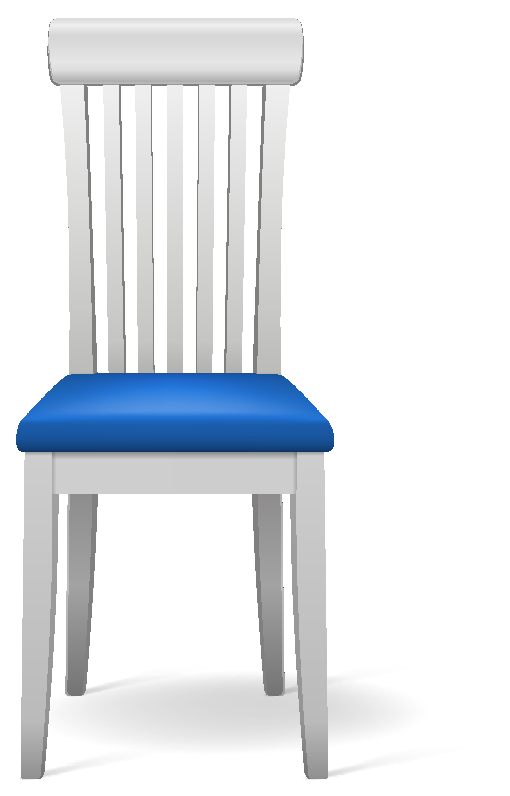
\includegraphics[height=1em]{chair/file.eps}}}$) \quad
  Tevfik Bultan \quad
  Chandra Krintz
}
\titlegraphic{\hfill
\includegraphics[width=2.25cm]{ucsbseal_cmyk.pdf}}

\begin{document}
\maketitle

\metroset{numbering=none}
\begin{frame}<beamer>[noframenumbering]
  \frametitle{Outline}
  \tableofcontents
\end{frame}
\metroset{numbering=fraction}

\section{Motivation}
\begin{frame}{What is low-level software? Why should we analyze it?}
Low-level software:
\begin{itemize}[<+->]
\item Drivers
  \begin{itemize}
  \item Interacts with intricate OS APIs and require preserving subtle invariants
  \item Not locking locks twice, not writing to a port after closing it, etc.
  \end{itemize}
\item Avionics software
  \begin{itemize}
  \item No undefined behavior: integer overflows, out of bounds accesses, etc.
  \item Uses a subset of the language, e.g. no dynamic allocation, no recursion\footcite{cousot2007varieties}
    \begin{itemize}
    \item Easier to analyze
    \end{itemize}
  \end{itemize}
\item They have strong reliability requirements
  \begin{itemize}
  \item with unpleasant consequences\iftoggle{labdemo}{: BSoD, data loss, Arianne~5, Heartbleed, Patriot missile}{}
  \end{itemize}
\end{itemize}
\end{frame}

\AtBeginSection[]
{
  \metroset{numbering=none}
  \begin{frame}<beamer>[noframenumbering]
    \frametitle{Outline}
    \tableofcontents[currentsection]
  \end{frame}
  \metroset{numbering=fraction}
}

\only<beamer>{ % all template changes are local to this group.
  \nottoggle{labdemo}{
    \setbeamertemplate{navigation symbols}{}
    \begin{frame}[plain]
      \begin{tikzpicture}[remember picture,overlay]
        \node[at=(current page.center)] {
          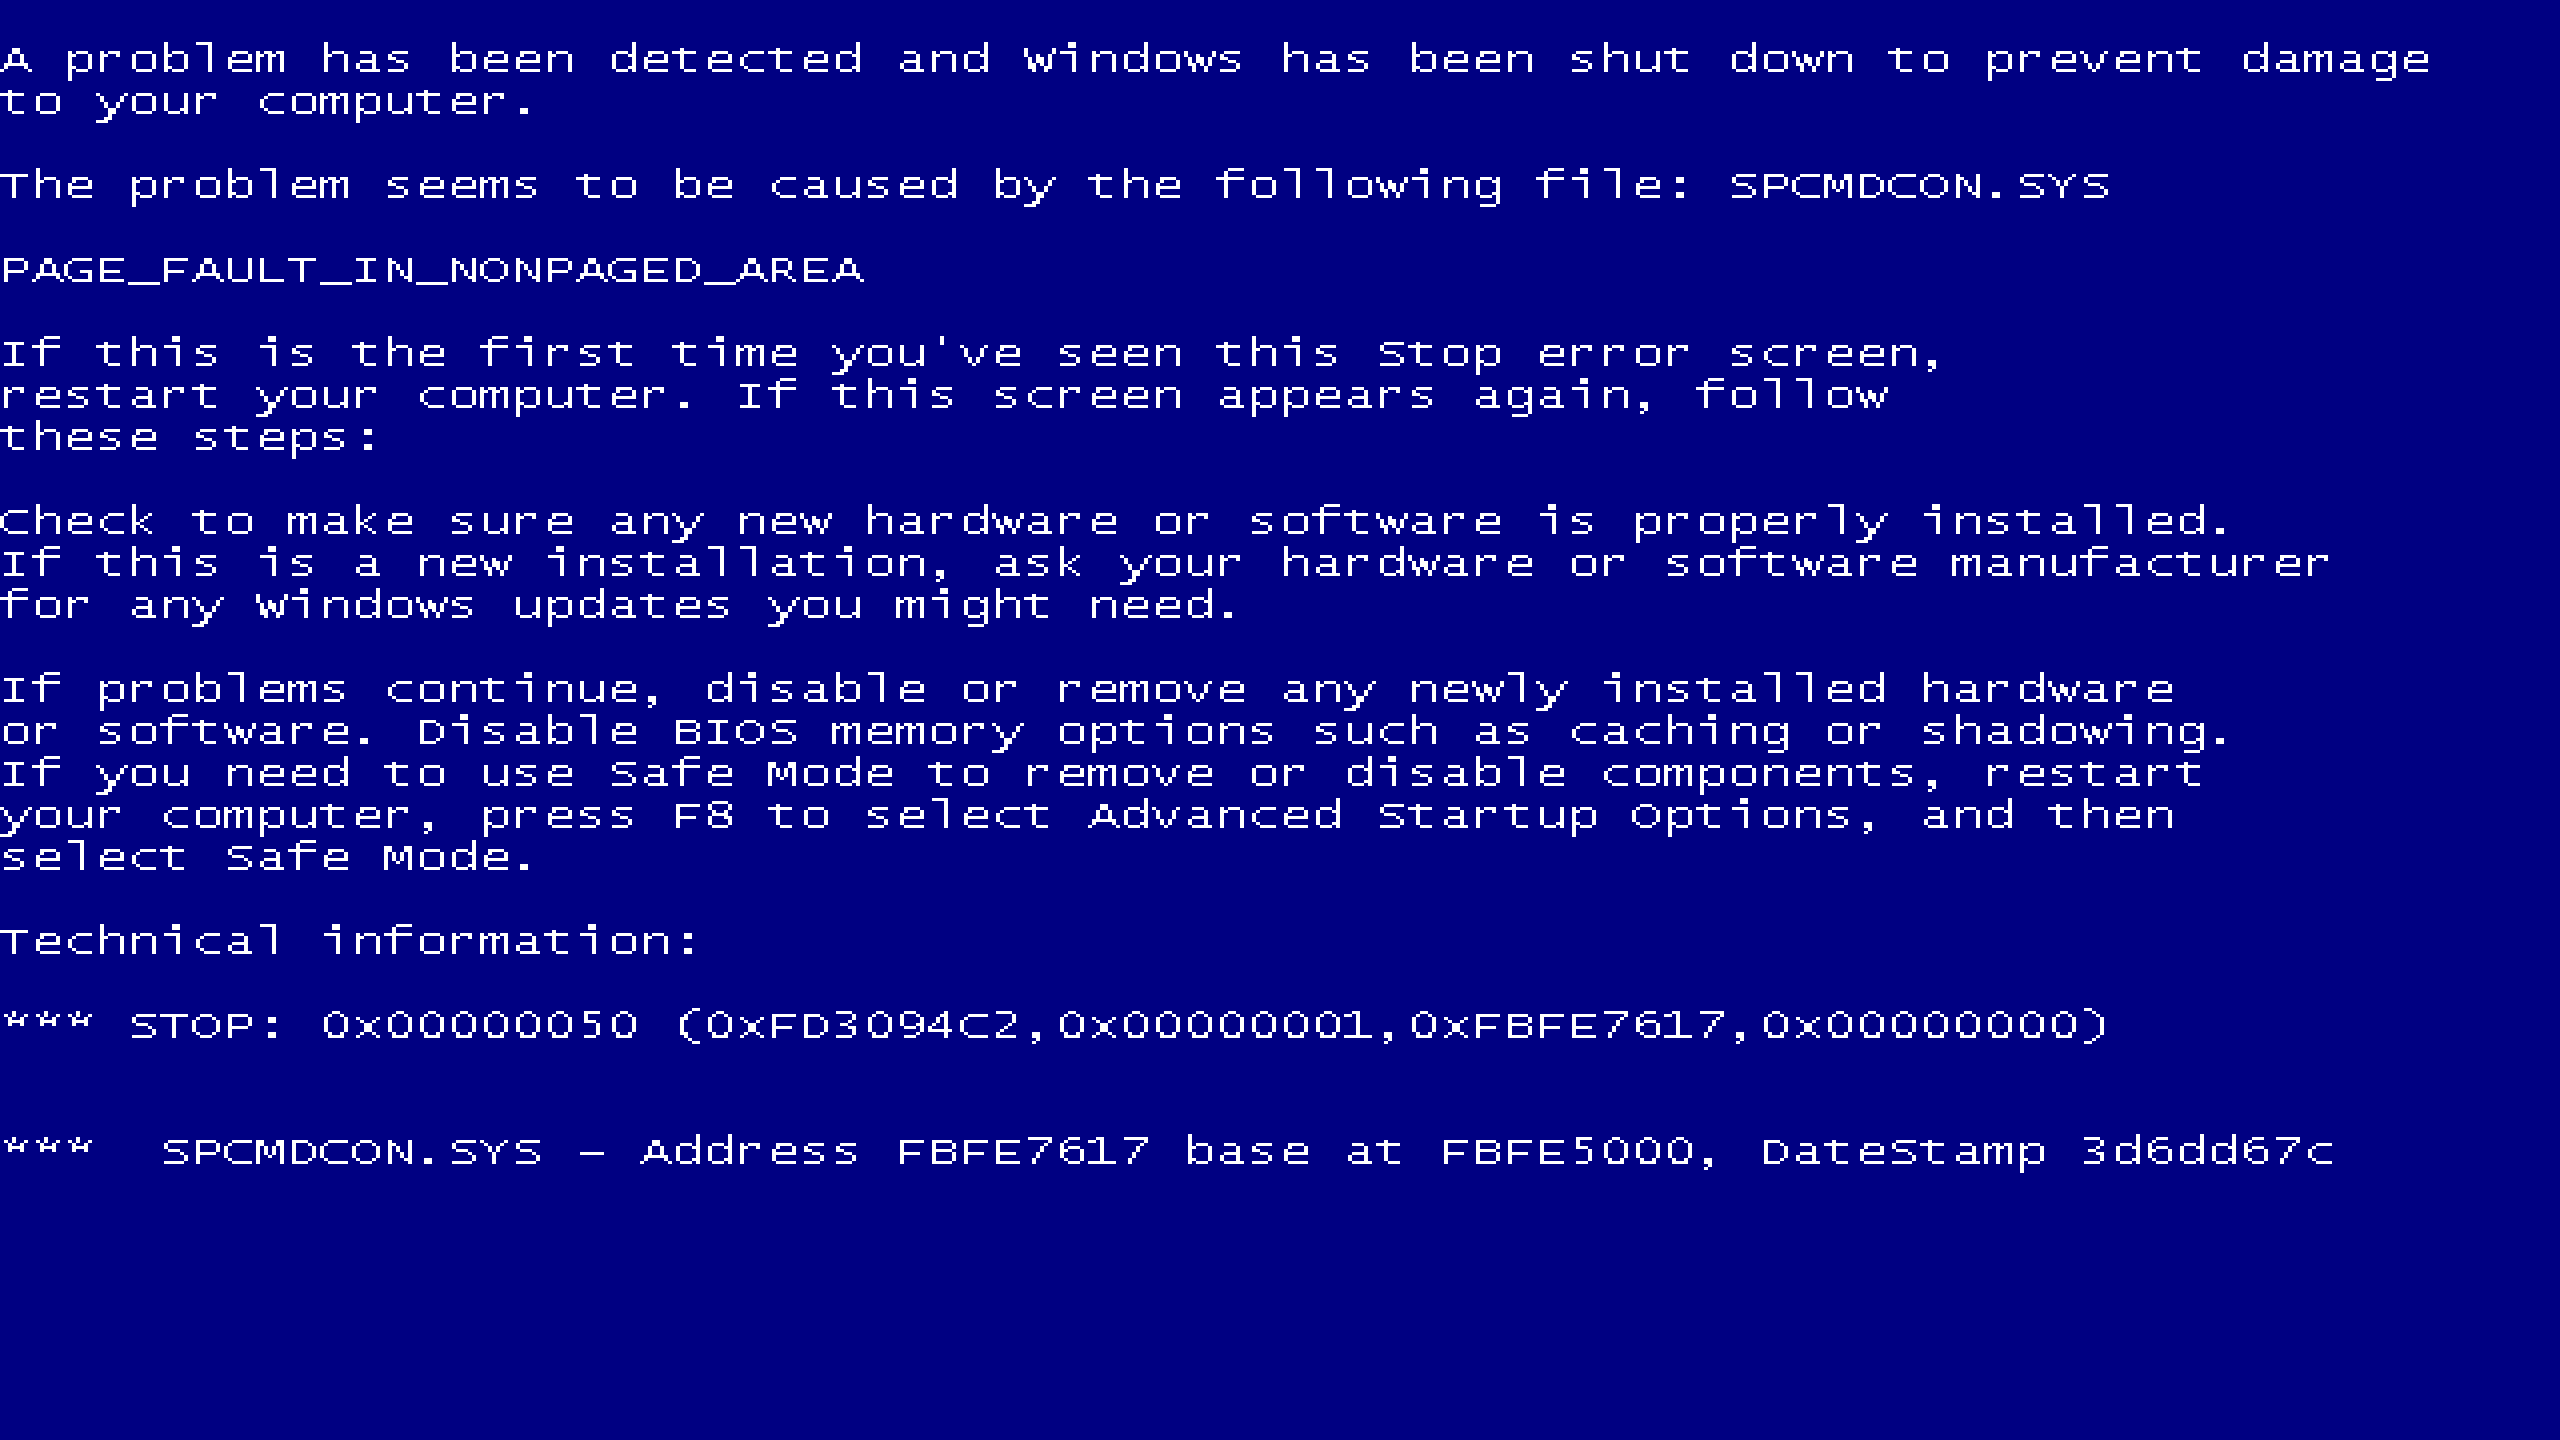
\includegraphics[width=\paperwidth]{material/bsod_resized.png}
        };
      \end{tikzpicture}
      % \sound[autostart,inlinesound]{foo}{beep.wav}
      \pause
      \Put(10,10){
\includegraphics[width=0.4\textwidth]{material/heartbleed.pdf}}\pause
      \Put(180,200){
\includegraphics[width=0.4\textwidth]{material/formal-verification-as-a-sinking-airplane.png}}\pause
      \Put(210,-100){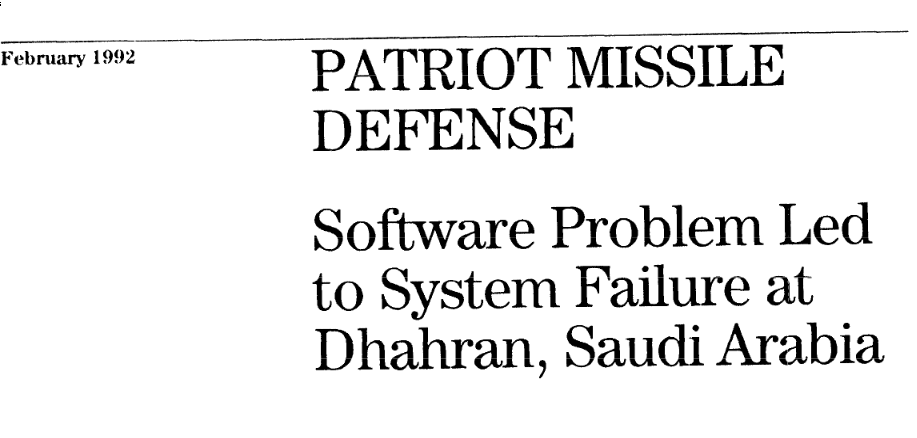
\includegraphics[width=0.5\textwidth]{material/us-govt-patriot-missile.png}}
    \end{frame}
  }{
    \addtocounter{framenumber}{1}
  }
}

\only<handout>{
  \addtocounter{framenumber}{1}
}

\section{Abstract interpretation}

\begin{frame}{Abstract interpretation}
  \begin{itemize}[<+->]
  \item Introduced by Cousot and Cousot in 1977 for a flow-chart language \footcite{cousot1977abstract}
  \item Can be designed systematically using math\footcite{cousot1979systematic}
  \item Expanded to be used with different kinds of semantics \footcite{schmidt1998trace,schmidt2009abstract,van2010abstracting,van2012systematic}
  \item General idea: Create an \emph{abstract} interpreter that
    overapproximates the \emph{concrete} interpreter's behavior
    soundly (captures all behavior)
    \begin{itemize}
    \item and abstract interpreter terminates 
    \end{itemize}

  \end{itemize}
\end{frame}

\begin{frame}[fragile]{Programs' executions as state transition systems}
  \footnotesize
  \begin{columns}[T]
    \begin{column}{0.45\textwidth}
      We want to show that division on line 3 is always exact in this program:

      \begin{lstlisting}[language=Java,numbers=left,mathescape,basicstyle={\footnotesize\ttfamily}]
x := random;
while (x mod 2 == 0) {
  x := x / 2;
  x := x + 1;
}
y := 2;
$$
\end{lstlisting}
\begin{itemize}
\item<2-> We can represent the program's execution as a state transition system
\item<10-> We are interested in all the values \texttt{x} can take at line 3
\item<11-> There are infinitely many states!
\end{itemize}
    \end{column}
    \begin{column}{0.5\textwidth}
    \multiinclude[<+>][start=1,format=pdf,graphics={height=0.9\textheight}]{fig/concrete-sem}
    \end{column}

  \end{columns}
\end{frame}

\begin{frame}[fragile]{Collecting semantics \& abstraction}
  \footnotesize
  \begin{columns}[T]
    \begin{column}{0.4\textwidth}
      \begin{itemize}
      \item We are interested in values \texttt{x} takes
      \item<9-> Specifically, its parity
      \item<15-> With this \emph{abstraction} we have a finite transition system
      \end{itemize}
      \begin{lstlisting}[language=Java,numbers=left,mathescape,basicstyle={\footnotesize\ttfamily}]
x := random;
while (x mod 2 == 0) {
  x := x / 2;
  x := x + 1;
}
y := 2;
$$
\end{lstlisting}
    \end{column}
    \begin{column}{0.6\textwidth}
      \only<beamer>{\multiinclude[<+>][start=1,format=pdf,graphics={height=0.9\textheight}]{fig/adhoc-lattice}}
      \only<handout>{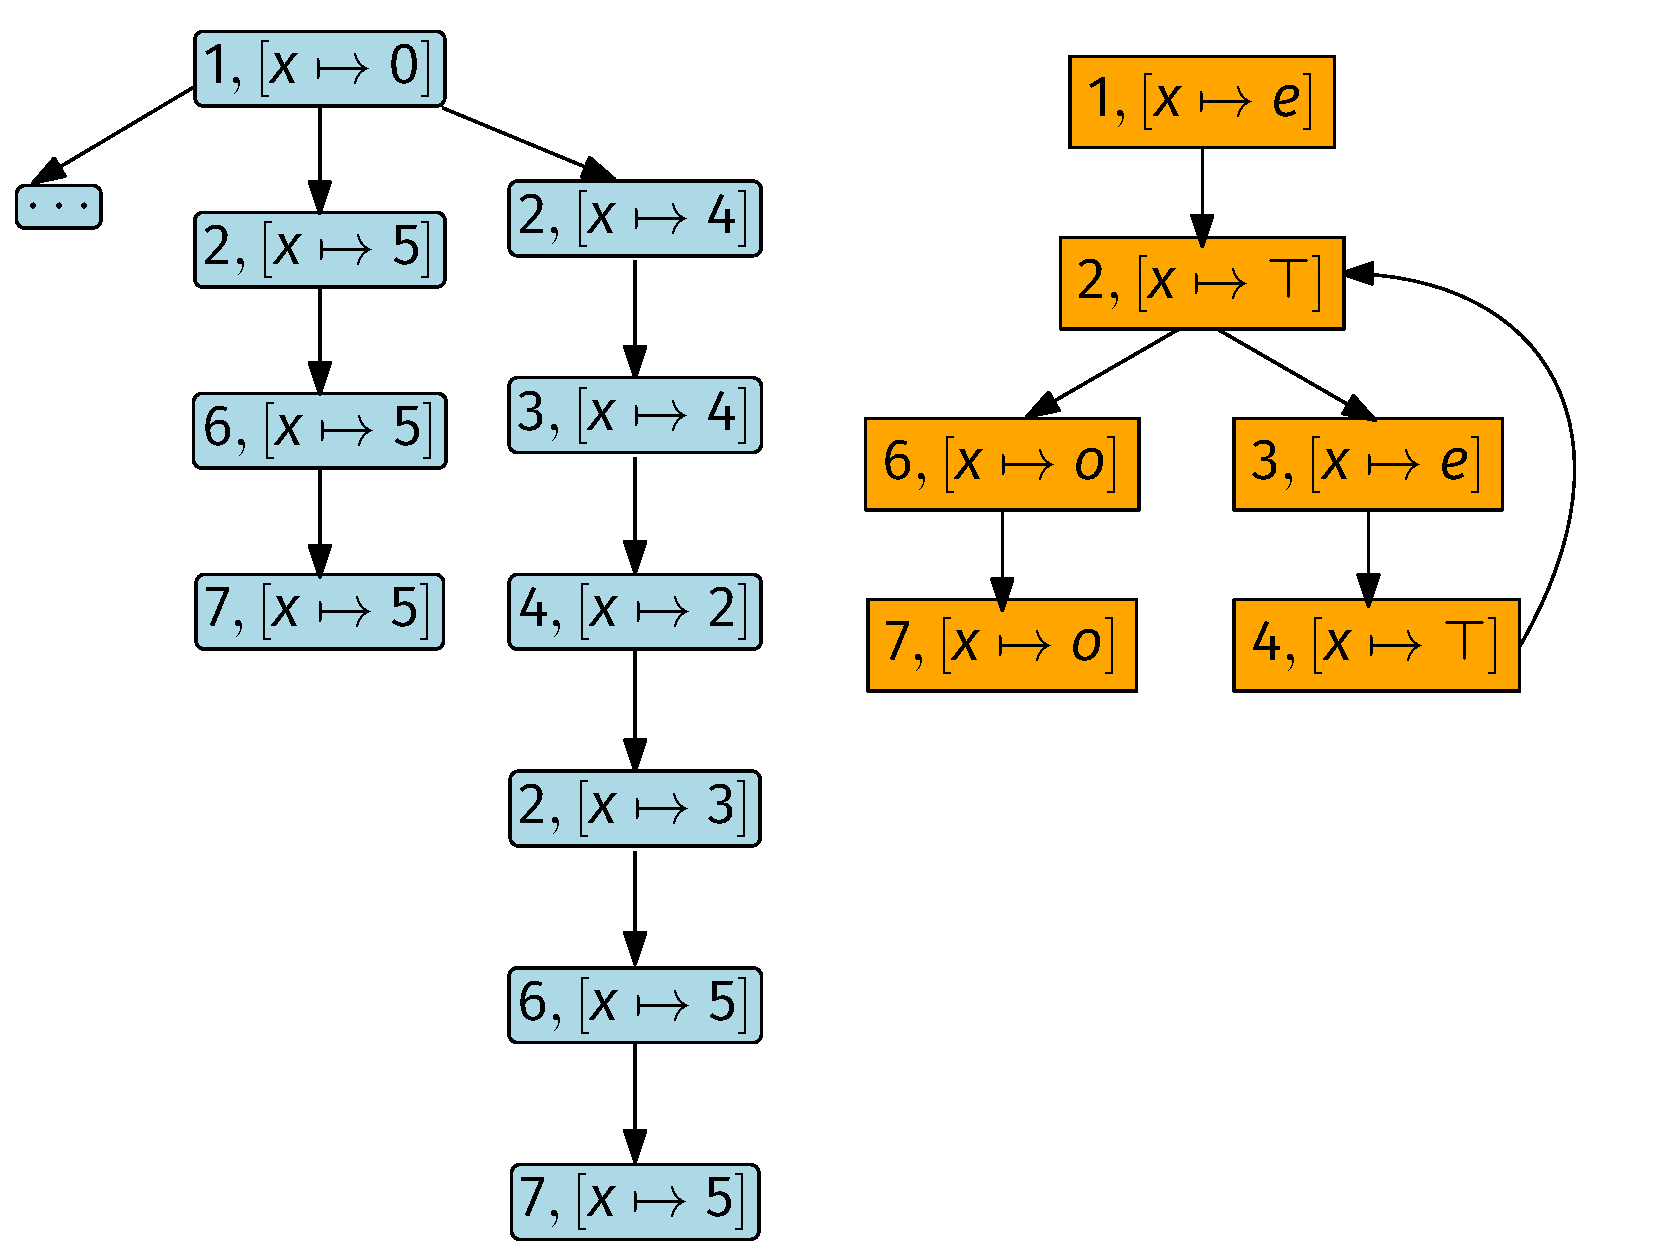
\includegraphics[height=0.9\textheight]{fig/adhoc-lattice-15.pdf}}
    \end{column}
  \end{columns}
\end{frame}

\begingroup
\small
\begin{frame}{Lattices and Order Theory}
  \begin{columns}[T]
  \begin{column}{0.6\textwidth}
  \begin{itemize}[<+->]
  \item Any powerset $\mathcal{P}(S)$ of a set $S$ has an interesting structure:
     $S$ is the largest set,
     $\emptyset$ is the smallest set,
     $\cup$, $\cap$ determine $\subseteq$
  \item A lattice $(L, \sqcup, \sqcap, \sqsubseteq)$ generalizes this notion. It is a partially ordered set (poset) with:
    \begin{itemize}\footnotesize
    \item a least upper bound (join) operation $\sqcup: L \times L \to L$ (similar to $\cup$)
    \item a greatest lower bound (meet) operation $\sqcap: L \times L \to L$ (similar to $\cap$)
    \item $\sqcup, \sqcap$ determine the partial order $\sqsubseteq$ (similar to $\subseteq$)
    \end{itemize}
  \item A bounded lattice has a least element $\bot$, (bottom)
    and greatest element $\top$ (top)
  \end{itemize}
  \end{column}
  \begin{column}{0.4\textwidth}
    \begin{figure}[h]
    \centering
    \begin{tikzpicture}[x=2cm, y=1.5cm]
      \node(top)at (1,3){$\textcolor<6>{mLightBrown}{\{+,-,0\} = \top}$} ;
      \node(pm)at (1,2){$\{+,-\}$} ;
      \node(mz)at (2,2){$\{-,0\}$} ;
      \node(pz)at (0,2){$\textcolor<3>{mLightBrown}{\{+,0\}}$} ;
      \node(p)at (0,1){$\{+\}$} ;
      \node(m)at (2,1){$\{-\}$} ;
      \node(z)at (1,1){$\textcolor<4>{mLightBrown}{\{0\}}$} ;
      \node(bot)at (1,0){$\textcolor<6>{mLightBrown}{\emptyset = \bot}$} ;
      \draw(top)--(pm);
      \draw(top)--(mz);
      \draw(top)--(pz);
      \draw(pm)--(p);
      \draw(pm)--(m);
      \draw(mz)--(m);
      \draw[onslide={<6> draw=mLightBrown, line width=1.2pt}](mz)--(z);
      \draw[onslide={<3> draw=mLightBrown, line width=1.2pt}](pz)--(p);
      \draw[onslide={<3,6> draw=mLightBrown, line width=1.2pt}](pz)--(z);
      \draw(p)--(bot);
      \draw(m)--(bot);
      \draw(z)--(bot);
    \end{tikzpicture}
    \caption{\footnotesize Hasse diagram of a sign lattice, built from $\pw(\{+,-,0\})$}
  \end{figure}
  % \only<4>{\begin{figure}[t]
  %   \centering
  %   \begin{tikzpicture}[x=1.25cm, y=1.25cm]
  %     \node(top)at (0,1){$\top$} ;
  %     \node(e)at (-1,0){$e$} ;
  %     \node(o)at (1,0){$o$} ;
  %     \node(bot)at (0,-1){$\bot$} ;
  %     \draw(top)--(o)--(bot);
  %     \draw(top)--(e)--(bot);
  %   \end{tikzpicture}
  %   \caption{Hasse diagram of an even/odd lattice}
  % \end{figure}}
  \end{column}
  \end{columns}
\end{frame}
\endgroup % footnotesize

\begingroup
\footnotesize
\begin{frame}{Relating lattices}
  \begin{columns}[T]
    \begin{column}{0.7\textwidth}
    \begin{itemize}
    \item There is a relationship between $\mathit{Parity}$ and
      $\mathcal{P}(\mathbb{Z})$:\vspace{-0.8em}
      \begin{align*}
        \uncover<2->{
        \alpha : \mathcal{P}(\mathbb{Z}) & \monarrow \mathit{Parity} \\
        \gamma : \mathit{Parity} & \monarrow \mathcal{P}(\mathbb{Z})
                                   }
      \end{align*}\vspace{-3em}
      \begin{align*}
        \uncover<3->{\alpha(S) & = \bigsqcup\limits_{z \in S}
        \begin{cases}
          o & z \text{ odd}\\
          e & z \text{ even}
        \end{cases}}\\
        \uncover<4->{\gamma(\top) & = \mathbb{Z}, \gamma(\bot) = \emptyset \\
        \gamma(o) & = \{z \in \mathbb{Z} \mid z \text{ odd} \} \\
        \gamma(e) & = \{z \in \mathbb{Z} \mid z \text{ even} \}}
      \end{align*}\vspace{-2em}
    \end{itemize}
  \end{column}
  \begin{column}{0.25\textwidth}
    \begin{figure}
      \centering
      \footnotesize
      \begin{tikzpicture}[x=1.25cm, y=1.25cm]
        \node(top)at (0,1){$\top$} ;
        \node(e)at (-1,0){$e$} ;
        \node(o)at (1,0){$o$} ;
        \node(bot)at (0,-1){$\bot$} ;
        \draw(top)--(o)--(bot);
        \draw(top)--(e)--(bot);
      \end{tikzpicture}\\[0.5em]
      \onslide<3->{$\alert<3>{\alpha(4) + \alpha(-7) = e + o = o}$}
      \caption{\footnotesize $\mathit{Parity}$ domain}
    \end{figure}
  \end{column}
\end{columns}\vspace{-1em}
\begin{itemize}
    \item<5-> $\alpha$ and $\gamma$ are \emph{sound}: we don't leave anything behind when we go abstract then come back to the concrete
    \item<6-> $\alpha$ and $\gamma$ are kind of like inverses, though
      there is some information loss
    \item<7-> oftentimes $\alpha$ is chosen to be the \emph{best possible} function to pair
      with $\gamma$ in a certain sense
    \item<8-> This relationship is known as a \alert{\emph{Galois Connection}}
\end{itemize}
\end{frame}
\endgroup

\begingroup
\small
\begin{frame}{Galois Connections}
  \[ \textcolor<2->{gray}{\forall c \in \mathit{Concrete}, a \in \mathit{Abstract}.\, c \subseteq \gamma(a) \iff \alpha(c) \sqsubseteq a} \]
  \pause
  or, equivalently,
  \[ \tikzmark{ma}\textcolor<1,7->{gray}{\alpha, \gamma \text{ monotone}}\tikzmark{mb} \qquad \tikzmark{a}\textcolor<1,4-6,10->{gray}{c \subseteq \gamma(\alpha(c))}\tikzmark{b} \qquad \tikzmark{ra}\textcolor<1,4-9>{gray}{\alpha(\gamma(a)) \sqsubseteq a\tikzmark{rb}} \]
  \pause
  \vspace*{-1em}
  \begin{tightcenter}
   \begin{tikzpicture}
     \draw[fill=lightblue] (0,0.25) ellipse (1.75cm and 1.75cm);
     \node at (0,2.33) {$\mathcal{P}(\mathbb{Z})$};
     \node at (5.5,1.5) {$\mathit{Parity}$};

     \node(top)at (5.5,1){$\top$} ;
     \node(e)at (4.5,0){$e$} ;
     \node(o)at (6.5,0){$o$} ;
     \node(bot)at (5.5,-1){$\bot$} ;
     \draw(top)--(o)--(bot);
     \draw(top)--(e)--(bot);

     \node (z) at (0,1.75) {$\mathbb{Z}$};
     \node (evens) at (-.75,1) {$evens$};
     \node (odds) at (.75,1) {$odds$};
     \node (two) at (0,-0.5) {$\{ 2 \}$};
     \node (empty) at (0,-1.0) {$\emptyset$};

     \draw<6,8-9>[->] (two) to [bend right] node [midway, below] {$\alpha$} (e) ;
     \draw<5-6>[->] (empty) to [bend right] node [pos=0.6, above] {$\alpha$} (bot) ;
     \draw<9,11->[->] (e) to [bend right] node [midway, above] {$\gamma$} (evens);
     \draw<12->[->] (evens) to [bend right] node [pos=0.6, above] {$\alpha$} (e);

   \end{tikzpicture}
 \end{tightcenter}

 \begin{tikzpicture}[overlay, remember picture]
   \draw<7-9>[draw=mLightBrown, line width=1.1pt] ($(a)+(-.1em,-.4em)$) rectangle ($(b)+(0.1em,1em)$);
   \draw<7-9>[draw opacity=0] (a) to node [midway, below, yshift=-.5em] {$\alpha$ is sound} (b);
   \draw<4-6>[draw=mLightBrown, line width=1.1pt] ($(ma)+(-.1em,-.4em)$) rectangle ($(mb)+(0.1em,1em)$);
   %\draw<4>[draw opacity=0] (ma) to node [midway, below, yshift=-.5em] {$\alpha$ is sound} (mb);
   \draw<10-12>[draw=mLightBrown, line width=1.1pt] ($(ra)+(-.1em,-.4em)$) rectangle ($(rb)+(0.1em,1em)$);
   %\draw<11>[draw opacity=0] (ra) to node [midway, below, yshift=-.5em] {$\alpha$ is sound} (rb);
 \end{tikzpicture}
\end{frame}
\endgroup

\begin{frame}[fragile]{Safe simulations}
  \small
  \vspace{-1em}
  \begin{itemize}[<+->]
  \item Run the concrete machine and the abstract machine in lockstep
  \item Taking a step in both \abscolor{abstract} and \concolor{concrete} machines should result in a new \emph{safe} pair of states
    \uncover<6->{\alert<7>{($\alpha \circ F \sqsubseteq \abst{F} \circ \alpha$)}}
  \begin{tightcenter}
    \begin{tikzcd}[execute at end picture={
        \only<beamer>{
      \onslide<3>{\node(o1)[fill=gray,opacity=0.1,fit=(ea.north west) (eb.north east) (eb.south east) (ea.south west)]{};}
      \onslide<4>{\node(o2)[fill=gray,opacity=0.1,fit=(aa.south west) (ea.north east)]{};}
      \onslide<5>{\fill[gray,opacity=0.1] (aa.north west) -- (ab.north east) -- (ab.south east) -- (aa.south west) -- cycle;}
      \onslide<6>{\node(o3)[fill=gray,opacity=0.1,fit=(ab.south west) (eb.north east)]{};}
      }
    },ampersand replacement=\&]
       \& |[alias=ea]| \concolor{\alt<3->{\varsigma}{x \mapsto 6}} \arrow[r, "\alt<3->{F}{x := x / 2}", squiggly] \arrow[dd, "\alpha", dotted] \& |[alias=eb]| \concolor{\alt<3->{\varsigma'}{x \mapsto 3} \arrow[d, "\alpha", dotted]} \\
    \&  \& \abscolor{\alt<3->{\alpha(\varsigma')}{x \mapsto o} } \arrow[d, "\sqsubseteq", dashed] \\
      \& |[alias=aa]| \abscolor{\alt<3->{\alpha(\varsigma)}{x \mapsto e}} \arrow[r,  "\alt<3->{\abst{F}}{x := x / 2}", squiggly] \& |[alias=ab]| \abscolor{\alt<3->{\alpha(\varsigma)'}{x \mapsto \top} }
    \end{tikzcd}
    \only<beamer>{
    \begin{tikzpicture}[remember picture, overlay,
      every node/.append style = { align = center, minimum height = 10pt,fill=gray,opacity=0.1,text opacity=1}]
      \onslide<3>{\node[left=6cm, text width=4cm](){\textcolor{gray}{\textsf{\footnotesize Program executing state $\varsigma$ transitions to state $\varsigma'$}}};}

      \onslide<4>{\node[left=6cm, text width=4cm](){\textcolor{gray}{\textsf{\footnotesize $\alpha(\varsigma)$ abstracts $\varsigma$}}};}

      \onslide<5>{\node[left=6cm, text width=4cm](){\textcolor{gray}{\textsf{\footnotesize Abstract state $\alpha(\varsigma)$ transitions to $\alpha(\varsigma)'$}}};}

      \onslide<6>{\node[left=6cm, text width=4cm](){\textcolor{gray}{\textsf{\footnotesize $\alpha(\varsigma)'$ covers $\alpha(\varsigma')$ thus is a safe counterpart for $\varsigma'$}}};}
    \end{tikzpicture}
    }
   \end{tightcenter}

   \vspace{-1em}
   \item<8> By induction, starting from an initially-safe pair of states we will soundly cover every possible path through the program
 \end{itemize}
\end{frame}

\begin{frame}{Computing fixpoints\footcite{kleene_stephen_cole_introduction_1952,tarski1955lattice,cousot1979constructive}}
  \begin{columns}
    \begin{column}{0.8\textwidth}
      \begin{thm}[Kleene-Tarski fixed point theorem]
        If $L$ is a complete lattice and $F: L \monarrow L$ then $\forall x \in L$, $\lfp_x F$ exists and
        \[
          \lfp_x F = \bigsqcup \Set{F^n(x) \vert n \in \nats}.
        \]
      \end{thm}

      \uncover<3->{Moreover, if $L$ is Noetherian (has no infinite chains), $\exists n. \lfp_x F = x \sqcup F(x) \sqcup F(F(x)) \sqcup \ldots \sqcup F^n(x)$.}
    \end{column}
    \begin{column}{0.2\textwidth}\footnotesize
      \begin{tikzcd}
        \alert<2>{x^* = F(x^*)} \\
        \vdots \arrow[u, no head] \\
        x \sqcup F(x) \sqcup F(F(x)) \arrow[u, no head] \\
        x \sqcup F(x) \arrow[u, no head] \\
        x \arrow[u, no head]
      \end{tikzcd}
    \end{column}
  \end{columns}
\end{frame}

\begin{frame}{Widening}
  \small
  \begin{columns}
    \begin{column}{0.75\textwidth}
      Fixpoint computation doesn't terminate on infinitely high lattices.\\
      \uncover<2->{A widening operator $\widen : A \times A \to A$ overapproximates join and}
      \begin{itemize}      
      \item<2-> accelerates fixpoint computation
      \item<3-> ensures termination even in an infinitely high lattice
      \item<4-> we make only finitely many jumps on a chain to converge
  \end{itemize}\vspace{-0.3em}
  \uncover<5->{
    \begin{exampleblock}{\small Example: a widening operator on intervals}
      \vspace{-0.8em}
      \begin{itemize}\footnotesize
      \item $[1,1] \widen [2,2] \widen [3,3] \widen \ldots \to [1, \infty]$
      \item $[1,5] \widen [0,5] \widen [-1,5] \widen \ldots \to [-\infty, 5]$
      \end{itemize}
    \end{exampleblock}
    }
\end{column}
\begin{column}{0.2\textwidth}\footnotesize
  \begin{onlyenv}<beamer>
    \begin{onlyenv}<-2>
    \[\begin{tikzcd}[ampersand replacement=\&]
      \alert<1>{\vdots} \& \\
      \alert<1>{a_3} \arrow[u, no head] \& \\
      \alert<1>{a_2} \arrow[u, no head] \& \\
      \alert<1>{a_1} \arrow[u, no head] \&
    \end{tikzcd}\]
  \end{onlyenv}
  \end{onlyenv}\tiny
  \begin{onlyenv}<3->
    \begin{tikzcd}[ampersand replacement=\&]
      \& \alert<4>{w_n}=w_{n-1} \widen a_n \\
      \& \vdots \arrow[u, no head] \\
      \alert<3>{\vdots} \textcolor<2>{mLightBrown}{\arrow[ruu, no head]} \& \alert<4>{w_3} = w_2 \widen a_3 \arrow[u, no head] \\
      \alert<3>{a_3} \textcolor<2>{mLightBrown}{\arrow[ru, no head]} \arrow[u, no head] \& \alert<4>{w_2} = w_1 \widen a_2 \arrow[u, no head] \\
      \alert<3>{a_2} \textcolor<2>{mLightBrown}{\arrow[ru, no head]} \arrow[u, no head] \&  \\
      \alert<3>{a_1}=\alert<4>{w_1} \textcolor<2>{mLightBrown}{\arrow[ruu, no head]} \arrow[u, no head] \&
    \end{tikzcd}
  \end{onlyenv}
\end{column}
\end{columns}
\uncover<6->{Widening operators are more general than Galois Connections to finite lattices\footcite{cousot92comparing}}

\end{frame}

\begin{frame}{Previous work on improving/designing abstract interpreters}
  \begin{itemize}
  \item Control flow analysis, $k$-CFA\footcite{shivers1991control}
  \item Abstract garbage collection\footcite{might2006improving}
  \item Widening for control flow\footcite{hardekopf2014widening}
  \item Monadic abstract interpreters\footcite{sergey2013monadic,darais2015galois}
  \end{itemize}

  \note{CFA constructs CFG dynamically. Abstract GC improves precision by removing inaccessible objects. AAM gives a systematic way to abstract certain semantics. Widening for control flow separates control flow sensitivity from rest of the analysis. Monadic a.i. factors that stuff into monads}
\end{frame}

\begin{frame}{Relationship with model checking}
  \begin{itemize}[<+->]
  \item Abstract interpretation links model
    checking and a certain kind of data flow analysis
    \footcite{schmidt1998program,schmidt1998data}
  \item There's a mechanical way to transform any bit-vector-based,
    iterative data flow analysis to a modal $\mu$-calculus formula
    \begin{itemize}
    \item
      $live(pp) = used(pp) \cup (notModified(pp) \cap (\bigcap_{pp' \in
        \fn{Post}(pp)} live(pp')))$
      \vspace{.5em}
    \item
      $isLive(x) = \nu Z \,.\, isUsed(x) \vee (\neg isModified(x)
      \wedge \square Z)$
    \end{itemize}
  \item (Trace-based) abstract interpretation creates the finite model of the
    program at the desired precision level
    \begin{itemize}
    \item We will see something in the same vein in predicate abstraction
    \end{itemize}
  \end{itemize}
\end{frame}

\section{Predicate abstraction \& abstraction refinement}

\begin{frame}{Predicate abstraction}
  \begin{itemize}[<+->]
  \item Predicates can encode the invariants we want to preserve when accessing interfaces
    \begin{itemize}
    \item Such as not locking a locked lock, not using a resource after releasing it
    \item Useful for verifying that drivers use the OS API correctly
    \end{itemize}
  \item Proposed by Clarke et al. and Graf et al. for hardware verification\footcite{clarke1994model,graf1997construction}
  \item Main idea: our abstract domain is a finite set of predicates $\Set{\phi_i,\, 1 \le i\le n}$ over states
  \item Use model checkers/theorem provers to compute reachability
  \end{itemize}
\end{frame}

\begin{frame}{Counterexample-Generated Abstraction Refinement (CEGAR)\footcite{clarke2003counterexample,ball2001automatic,ball2001automatically}}
  \small
  % \begin{itemize}[<+->]
  % \item Choosing the correct predicates is tricky and tedious
  % \item When proving safety using the current abstraction fails, compute a counterexample using backwards semantics ($\fn{Pre}$) and a model checker to find a path it fails
  % \item Add the counterexample to the set of predicates and try again
  % \item Proposed by Clarke et al.\footcite{clarke2003counterexample}. Extended by Ball et al. to support C programs for SLAM project\footcite{ball2001automatic,ball2001automatically}
  % \end{itemize}
  \begin{tightcenter}
    \multiinclude[<+>][start=1,format=pdf,graphics={width=0.7\textwidth}]{fig/cegar}
  \end{tightcenter}
  \note{Finding the correct predicates again and again is tedious, why not automate it?\\ }
  \note{During abstraction, we extract the predicates that affect/depend on parameters/globals/returns for each procedure, carry that as a signature and use it to create the Boolean program. SLAM is inter-procedural but it is not context sensitive\\}
  \note{Announce: An example is coming up}
\end{frame}

\begin{frame}{Predicate abstraction: Instrumentation code}
  \todo{Check again}
  \begingroup\footnotesize
  $\phi_1 = \texttt{\{state==Locked\}}$, $\phi_2 = \texttt{\{state==Unlocked\}}$

  \begin{itemize}[<+->]
  \item The code on the left is generated by a specification for using
    spin locks properly
  \item The code on the right is the predicate abstraction of the code on the left
  \end{itemize}
  \endgroup

  \begin{columns}[t]
    \begin{column}{0.45\textwidth}
      \lstinputlisting[language=C,mathescape]{lst/pred_instr.c}
    \end{column}
    \begin{column}{0.45\textwidth}
      \lstinputlisting[language=C,mathescape]{lst/pred_instr.bool}
    \end{column}
  \end{columns}
\end{frame}

\begin{frame}{\alt<5->{Abstraction refinement}{Predicate abstraction: The actual program}}
  \todo{Make the model checking part pictorial by putting a CFG and analyzing it}
  \begingroup\footnotesize\vspace{-0.7em}
  $\phi_1 = \texttt{\{state==Locked\}}$, $\phi_2 = \texttt{\{state==Unlocked\}}$\vspace{-1.7em}
  \begin{columns}[t]
    \begin{column}{0.50\textwidth}
      \lstinputlisting[language=C,mathescape]{lst/pred_program.c}
    \end{column}\pause
    \begin{column}{0.50\textwidth}
      \begin{center}

      \only<beamer>{
        \only<3>{\lstinputlisting[language=C,mathescape]{lst/pred_program.bool}}
        }
        \only<4->{\lstinputlisting[language=C,mathescape]{lst/pred_program2.bool}}
        \begin{itemize}\footnotesize
        \item<5-> Send this program to the model checker to verify it
        \item<6-> The model checker finds a bad path (counterexample) try falsifying it using concrete reachability analysis% symbolic execution to obtain a refinement
        \item<7-> Refine with $\phi_3 = \texttt{\{nPackets==nPacketsOld\}}$, generated from the counterexample
        \end{itemize}
      \end{center}

    \end{column}
  \end{columns}
  \endgroup

  \note<1->{We instrument the code (automatically) based on the specification}
  \note<2->{We abstract away the statements \& guards not interacting with predicates}
  \note<2->{Let's clean the useless cruft}
  \note<3->{SLAM does a backwards abstract interpretation then uses forward concrete semantics. BLAST does the opposite.}
\end{frame}

\begin{frame}{Lazy abstraction\footcite{henzinger2002lazy}}
  \begin{itemize}[<+->]
  \item We don't need to analyze the whole program after refinement
  \item Lazy abstraction applies refinement to only the program states after the state initiating the refinement
    \begin{itemize}
    \item It computes a new smaller refined transition system after refinement
    \item Different states can have different predicate abstractions
    \end{itemize}
  \end{itemize}
\end{frame}

\begin{frame}{Other work in abstraction refinement}
  \begin{itemize}[<+->]
  \item Using Craig interpolants rather than weakest preconditions gives $3.8$-$17.7\times$ speedup over lazy abstraction on BLAST benchmarks\footcite{mcmillan2006lazy}
  \item Gulavani et al.\footcite{gulavani2006counterexample} use abstraction refinement to compute which widenings to delay
    \begin{itemize}
    \item They later on extend their technique to get more precise widenings by using interpolants\footcite{gulavani2008automatically}
    \end{itemize}
    \item Podelski et al.\footcite{podelski2007armc} show that abstraction refinement can be implemented using CLP by modifying Prolog's fact database on the fly
  \end{itemize}
\end{frame}

\section{Static analysis of control software}
\begin{frame}{What is challenging about control software?}
  Example: avionics software, nuclear plant rod controllers etc.

  \begin{itemize}[<+->]
  \item We want some strict requirements such as no integer overflows
    \begin{itemize}
    \item Requires reasoning about complex numerical relationships
    \end{itemize}
  \item Has multiple synchronous components
    \begin{itemize}
    \item Control part of the state is not as straightforward as sequential programs
    \item We need to figure out how to partition the state space to have a precise analysis
    \end{itemize}
  \item Has other restrictions making them a nice target for program analysis
    \begin{itemize}
    \item No dynamic memory allocation, no recursion, etc.
    \end{itemize}
  \end{itemize}

  \note{overflows are fine for Civ, not so fun when you're 10,000 ft up in the air\\}
  \note{we did the simple example, now we are ready for the complex one}
\end{frame}

\subsection{Dynamic state partitioning}
\begin{frame}{Partitioning the state of control programs}\small
  \todo{try giving an example or simplifying this in general}
  \begin{itemize}[<+->]
  \item Many control programs don't have a program counter like sequential programs
  \item Bultan et al.\footcite{bultan_model-checking_1999} propose a method to decompose the transition relation. Their method has 3 stages:
    \begin{enumerate}
    \item Convert an event-action language to DNF Presburger formulas
    \item Partition the state space by different valuations of selected control variables
      \begin{itemize}
      \item Also partition the state space by activation conditions of events
      \item Decompose the transition relation to have states in a single partition for the domain and the range of each transition formula
      \end{itemize}
    \item Apply only the relevant parts of the transition relation to each partition when computing a fixpoint
    \end{enumerate}
  \item They later on extend this technique to work on programs containing integers, Booleans, and enums\footcite{bultan_composite_2000}
  \end{itemize}
  \note{Their main contribution is symbolic model checking of infinite state systems}
  \note{They evaluate their technique by verifying properties of Bakery algorithm, ticket algorithm, bounded buffer producer-consumer, and a circular queue.}
  \note{In this work, they merge formulas from the same language together then apply simplification procedures per sublanguage separately}
\end{frame}

\begin{frame}{Dynamic state partitioning for automata\footcite{jeannet_dynamic_1999}}
  \begin{columns}
    \begin{column}{0.7\textwidth}
      \begin{itemize}[<+->]
      \item Jeannet et al. propose a technique to partition state space of an automaton with linear arithmetic constraints as guards
      \item First do a reachability analysis on the automaton's control structure to get an initial CFG
      \item Then partition each state according to the guards present in the program
        \begin{itemize}
        \item Partition a state according to a guard if the guard's condition also partitions the outgoing transitions
        \end{itemize}
      \item Do the analysis after splitting one node, repeat until verifying the program or no more splits are available
      \end{itemize}
    \end{column}

    \begin{column}{0.3\textwidth}
      \begin{figure}
        \centering
        
      \only<beamer>{\multiinclude[<+>][start=1,format=pdf,graphics={height=0.3\textheight}]{fig/state-partitioning}}
      \only<handout>{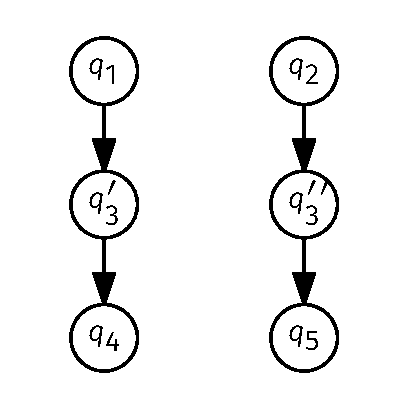
\includegraphics[height=0.3\textheight]{fig/state-partitioning-2.pdf}}
      
      \caption{Splitting happens only if it leads to partitioning outgoing edges}
    \end{figure}

    \end{column}
  \end{columns}
  \note{according to Jeannet, their partitioning is finer than Bultan's}
\end{frame}

\begin{frame}{Other methods for partitioning the state}
  \begin{itemize}[<+->]
  \item Partitioning transfer functions of automata with Booleans and integers by representing the functions as a MTBDD\footcite{jeannet_representing_2002}
  \item Extending an abstract interpreter for sequential programs to parallel programs\footcite{mine2011static}
    \begin{itemize}
    \item Restrictions: threads and locks are statically known, reasonable for control~programs
    \item Partition the state space based on the state of threads (waiting on a lock $l$, yielding, ready) and state of locks (held by thread $t$, free)
    \item Refine interactions of threads by throwing away impossible configurations
    \end{itemize}
  \item Automatically extracting branch conditionals from CFG to construct binary decision trees to partition state space\footcite{chen2015binary}
  \end{itemize}
\end{frame}

\subsection{Combination of domains}
\begin{frame}{A plethora of domains}
  \footnotesize
  \begin{itemize}[<+->]
  \item Analyzing control software requires reasoning about complex numerical relationships
  \end{itemize}
  \begin{tightcenter}
  \begin{tabular}{lccc}
    \textbf{Domain} & \textbf{Constraints} & \textbf{Complexity} \\
    % Presburger formulas\footcite{bultan_model-checking_1999} & Presburger arithmetic & $ \bigO(2^{2^{2^{pn}}}) $ \\
    Polyhedra\footcite{cousot1978automatic} & \( \sum_{j} c_{ij}x_j \leq 0 \) & \alert<2>{$ \bigO(2^n)$} & \uncover<2->{Too expensive!} \\ \pause
    \alt<6>{\emph{Octagons}}{Octagons}\footcite{mine2004weakly} & \( \pm x \pm y \leq c \) & $ \bigO(n^3) $ \\
    Pentagons\footcite{logozzo2010pentagons} & \( x \in [a,b] \wedge x < y \) & $ \bigO(n^2) $ \\
    Gauges\footcite{venet2012gauge} & \( x \in \left[\sum_{j} a_{j}\lambda_j, \sum_{j} b_{ij}\lambda_j \right] \) & $ \bigO(n2^l) $ & \uncover<5->{\alert<5>{Works better with bounded loops}}
    %Arithmetic-geometric progressions\footcite{feret2005arithmetic} & \( x \mapsto ax + b \) & $ \bigO(n) $
  \end{tabular}
  \end{tightcenter}
  \begin{itemize}
  \item<4-> Also: congruences, floating-point versions\footcite{mine2004relational}, \alt<6>{\emph{arithmetic-geometric progressions}}{arithmetic-geometric progressions}\footcite{feret2005arithmetic} \ldots{}
  \item<6-> \alert{How do we combine the results of different domains?}
  \end{itemize}
  \vspace*{1em}
\note{We want to reason about different kinds of constraints. Most expressive domains are too expensive. Some domains are designed to use the restrictions control software has: gauges--avionics. We want octagons to help with relational stuff, progressions to see how fast values grow with a clock tick; communication would help here}
\end{frame}

\begin{frame}[fragile]{Reduced products\footcite{cousot1979systematic}}
  \small
  \begin{figure}
    \raggedright
    \begin{subfigure}[b]{0.28\textwidth}\centering\tiny
      \[\begin{tikzcd}
        & \top &  \\
        \mathit{Null} \arrow[ru, no head] &  & \mathit{NotNull} \arrow[lu, no head] \\
        & \bot \arrow[ru, no head] \arrow[lu, no head] &
      \end{tikzcd}\]
      \caption{\small Nullity domain $\ns{Null}$}
    \end{subfigure}
    \begin{subfigure}[b]{0.25\textwidth}\centering\tiny
      \[\begin{tikzcd}
        & \top &  \\
        \mathit{Cyclic} \arrow[ru, no head] &  & \mathit{NotCyclic} \arrow[lu, no head] \\
        & \bot \arrow[ru, no head] \arrow[lu, no head] &
      \end{tikzcd}\]
      \caption{\small Cycle domain $\ns{Cyc}$}
    \end{subfigure}\pause
    \begin{subfigure}[b]{0.45\textwidth}\tiny
      \raggedright
      
      \[
        \begin{tikzcd}
 &  & \top &  \\
\only<2>{\alert{Cyc} \arrow[rru, no head]} & Null \arrow[ru, no head] & NotNull \arrow[u, no head] \arrow[rd, no head] & Acyc \arrow[lu, no head] \\
\only<2>{\alert{Null,Cyc} \arrow[u, no head] \arrow[ru, no head, crossing over]} & NotNull,Cyc \only<2>{\arrow[lu, no head, crossing over]} \arrow[ru, no head] & Null,Acyc \arrow[lu, no head, crossing over] \arrow[ru, no head, crossing over] & NotNull,Acyc \arrow[u, no head] \\
 &  & \bot \arrow[ru, no head] \arrow[u, no head] \arrow[lu, no head] \only<2>{\arrow[llu, no head]} & 
\end{tikzcd}
      \]
    \caption{\small \alt<3->{The reduced product of $Null$ and $Cyc$}{The Cartesian product $Null \times Cyc$}}
  \end{subfigure}
\end{figure}\vspace*{-1em}
\begin{itemize}
\item<4-> Reduced products have the same concretization. They prune unnecessary combinations
\item<5-> Optimal reduced products are not modular (new domains require ground-up design)
\item<6-> But iterative reductions can provide a modular implementation
\end{itemize}

\end{frame}

\begin{frame}{Iterative reductions\footcite{cousot2011reduced}}
  \small
  \begin{tightcenter}
    \multiinclude[<+->][start=1,format=pdf,graphics={height=0.3\textheight}]{fig/reduction}
  \end{tightcenter}
  \begin{itemize}
  \item A reduction operator $\rho: L \to L$ over a lattice $L$ is
    \begin{itemize}
    \item<2-> is a reductive $\rho(a) \sqsubseteq a$ operation
    \item<3-> that preserves concretization $\gamma \circ \rho = \gamma$ (is sound)
    \end{itemize}
  \item<4-> The communication of information between two domains is a reduction operator. Iteratively applying it until reaching a fixpoint is a reduction of the Cartesian product.
  \end{itemize}
\end{frame}

\begin{frame}{Reduction example: ASTRÉE's\footcite{cousot2005astree} Binary product abstract domain functor\footcite{cousot2006combination}}
  \todo{Add a picture}
  \begin{itemize}[<+->]
  \item $\dottimes : \mathcal{D \times D} \to \mathcal{D}$. It combines two domains and shares information between them automatically
  \item The information sharing is done by passing new constraints generated by some domains to others
  \item The constraints passed to $\mathcal{A \dottimes B}$ are passed to both $\mathcal{A}$ and $\mathcal{B}$
  \item The new constraints generated by $\mathcal{A}$ are passed to $\mathcal{B}$
  \item The refinement is acyclic to ensure termination (not to make widening unstable)
  \end{itemize}
\end{frame}

\begin{frame}{An example domain hierarchy from ASTRÉE\footcite{cousot2006combination}}
  \begingroup\tiny
  \begin{center}
    \begin{tikzcd}[ampersand replacement=\&]
      \& \alert<1>{\textsf{trace partitioning}} \arrow[d, no head] \&  \&  \&  \&  \\
      \& \alert<3>{\dottimes} \arrow[ld, no head] \arrow[rd, no head] \&  \&  \&  \&  \\
      \textsf{intervals} \&  \& \alert<3>{\dottimes} \arrow[ld, no head] \arrow[rd, no head] \&  \&  \&  \\
      \& \textsf{symbolic domain} \&  \& \alert<3>{\dottimes} \arrow[ld, no head] \arrow[rd, no head] \&  \&  \\
      \&  \& \textsf{octagons} \&  \& \alert<2>{\textsf{boolean partitioning}} \arrow[d, no head] \&  \\
      \&  \&  \&  \& \alert<3>{\dottimes} \arrow[ld, no head] \arrow[rd, no head] \&  \\
      \&  \&  \& \textsf{intervals} \&  \& \textsf{symbolic domain}
    \end{tikzcd}
  \end{center}
  \endgroup
  \note{Trace partitioning distinguishes between different traces up to current program point and keeps a couple domains below it}
  \note{Boolean partitioning splits the states for different values of a set of booleans, similar to predicate abstraction}
  \note{Binary product connects domains to get a partially reduced product, as explained above}
\end{frame}

\begin{frame}{Wrap-up}
  \begin{itemize}[<+->]
  \item Proving absence of errors in low-level programs is important
  \item Abstract interpretation is a framework for constructing sound program analyses by abstracting program behavior
  \item Predicate abstraction and abstraction refinement help proving that a (low-level) program uses APIs correctly
  \item Analyzing control software has some challenges. Two of them are:
    \begin{itemize}
    \item Partitioning of state space may not be as obvious: partition by guards in the program, control variables, etc.
    \item Combining different domains: reduced products help there
    \end{itemize}
  \end{itemize}
\end{frame}

\begin{frame}[standout]
  Thank you!
\end{frame}

\appendix

\begin{frame}{SIMPL\footnote{simple introductory made-up programming language} Syntax}
  \vspace{-2em}\only<handout>{\usebeamercolor*[fg]{normal text}}
  \small
  \begin{gather*}
    x,f \in \Var,\, b \in \bools,\, n \in \zahlen,\, \oplus \in \ns{BinOp},\,\Value = \bools \disunion \zahlen
  \end{gather*}\vspace{-2em}
  \begin{align*}
    fd \in \ns{FunDef} \eDEF & \alert<5>{\kw{def}\; f(\vo{x}) = s;\,\kw{return}\; e} \\
    e \in \Exp \eDEF & x \eOR n \eOR b \eOR e_1 \oplus e_2 \eOR \boxdot e \eOR \alert<3>{*x} \eOR \kw{random}  \\
    s \in \Stmt \eDEF & s;\,s \eOR \alert<2>{\kw{abort}} \\
    \eOR & \alert<4>{\kw{if}\, e\; s_1 \; \kw{else} \; s_2} \\
    \eOR & \alert<4>{\kw{while}\; e\; s} \\
    \eOR & \kw{let}\; x := e \;\kw{in}\;s \\
    \eOR & \alert<3>{\kw{letref}\; x := \kw{new}\;e \;\kw{in}\;s} \\
    \eOR & \alert<3>{e_1 \update e_2} \eOR x := e \\
    \eOR & \alert<5>{x := f(\vo{e})}
  \end{align*}
\end{frame}
\begin{frame}{SIMPL semantic domains}
  \begingroup\footnotesize We will use abstract machine semantics and represent the semantics of a program as a transition relation.\endgroup
\begin{align*}
    \varsigma \in \State & = \alert<1>{\Stmt^? \times \Env \times \Store \times \alert<2>{\Kont}} \\
    \rho \in \Env & = \Var \to \alert<3>{\Value} \\ % \alert<4>{\Value}^{\Var} \only<3>{\alert{= \Set{\rho : \Var \to \Value}}} \\
    \sigma \in \Store & = \alert<4>{\Addr} \to \alert<3>{\Value} \\ % \alert<4>{\Value}^{\alert<5>{\Addr}} \\
    \kappa \in \alert<5>{\Kont} & = \sTag{stmtK}{\Stmt \times \alert<5>{\Kont}} \\
                         & \disunion \sTag{whileK}{\Exp \times \Stmt \times \alert<5>{\Kont}} \\
                         & \disunion \sTag{retK}{\Var \times \Exp \times \Env \times \alert<5>{\Kont}} \\
                         & \disunion \sTag{haltK}
\end{align*}

\uncover<2>{Continuations represent \emph{the rest of computation}.}
\uncover<3>{Some parts of the state space are infinite}
\end{frame}

\begin{frame}{Some transition rules}
  \small
  \begin{itemize}
  \item $\varsigma \step \varsigma'$ is the transition relation%\footnote{Because of nondeterminism. One can also view it as a transition \emph{function} from a state to a set of states.}
  \item \(\eta_\varsigma : \Exp \to \Value \) is the per-state expression evaluation function
\item Current state: \(\varsigma = (so, \rho, \sigma, \kappa) \)
\item Next state: \( \varsigma' = (so', \rho', \sigma', \kappa') \) \pause
  \end{itemize}
  \footnotesize
  \[
  \begin{array}{llllll}
    so & \text{side condition} & so' & \rho' & \sigma' & {\kappa}' \\ \hline
    e_1 \update e_2 & & - & \rho & \sigma[\eta_\varsigma(e_1) \mapsto \eta_\varsigma(e_2)] & {\kappa} \\
    \kw{while}\; e\; s & \eta_\varsigma(e) = \true & - & \rho & \sigma & \sTag{stmtK}{(s, \sTag{whileK}{(e, s,\kappa)})} \\
    \kw{while}\; e\; s & \eta_\varsigma(e) = \false & - & \rho & \sigma & {\kappa} \\
    - & \kappa = \sTag{stmtK}{(s,\kappa_r)} & s & \rho & \sigma & {\kappa_r}
  \end{array}
  \]
\end{frame}

\begin{frame}{Collecting semantics}
  Abstract machine semantics gives us a state transition system $(\State, I, \step)$ where $\State$ is the set of states, $I \subset \State$ is the set of initial states, $\step \subset \State \times \State$ is the transition relation. \pause Let
  \[ F : \pw(\State) \alert<-3>{\monarrow} \pw(\State),\, F(X) = \Set{y \vert x \step y \wedge x \in X}. \]\pause

  F is monotonic: if $x \subseteq y$ then $F(x) \subseteq F(y)$

  $\lfp_I F = I \cup F(I) \cup F(F(I)) \cup \ldots $ is the set of reachable states.\pause

  \alert{$\lfp_I F$ is potentially infinite and requires infinitely many steps to compute!}
\end{frame}

\begin{frame}{Widening, detailed}
  \small
  \todo{Simplify}
  \begin{columns}
    \begin{column}{0.75\textwidth}
  A widening operator $\widen : A \times A \to A$ ensures convergence
  in a domain $A$ with infinite height. It has the following
  properties:\vspace{-0.3em}
  \begin{itemize}\footnotesize
  \item<2-> $\forall a_1, a_2 \in A, a_1 \sqcup a_2 \sqsubseteq a_1 \widen a_2$
  \item<2-> For any sequence $a_1, a_2, \ldots$, let $w_1 = a_1, \ldots, w_n = w_{n-1} \widen a_n$. Then, $a_i \sqsubseteq w_i$ and the chain $w_1, w_2, \ldots$ eventually stabilizes
  \end{itemize}\vspace{-0.3em}
  \uncover<5->{
    \begin{exampleblock}{\small Example: a widening operator on intervals}
      \vspace{-0.8em}
      \begin{itemize}\footnotesize
      \item $[1,1] \widen [2,2] \widen [3,3] \widen \ldots \to [1, \infty]$
      \item $[1,5] \widen [0,5] \widen [-1,5] \widen \ldots \to [-\infty, 5]$
      \end{itemize}
    \end{exampleblock}
    }
\end{column}
\begin{column}{0.2\textwidth}\tiny
  \uncover<2->{
    \begin{tikzcd}[ampersand replacement=\&]
      \& \alert<4>{w_n}=w_{n-1} \widen a_n \\
      \& \vdots \arrow[u, no head] \\
      \alert<3>{\vdots} \textcolor<2>{mLightBrown}{\arrow[ruu, no head]} \& \alert<4>{w_3} = w_2 \widen a_3 \arrow[u, no head] \\
      \alert<3>{a_3} \textcolor<2>{mLightBrown}{\arrow[ru, no head]} \arrow[u, no head] \& \alert<4>{w_2} = w_1 \widen a_2 \arrow[u, no head] \\
      \alert<3>{a_2} \textcolor<2>{mLightBrown}{\arrow[ru, no head]} \arrow[u, no head] \&  \\
      \alert<3>{a_1}=\alert<4>{w_1} \textcolor<2>{mLightBrown}{\arrow[ruu, no head]} \arrow[u, no head] \&
    \end{tikzcd}
  }
\end{column}
\end{columns}
\uncover<6->{Widening operators are more general than Galois Connections to finite lattices\footcite{cousot92comparing}}

\end{frame}


\begin{frame}{Abstracting Abstract Machines (AAM)\footcite{van2010abstracting,van2012systematic}}
  \only<beamer>{\only<1>{Here is our state, let's start by abstracting it pointwise}
  \only<2>{We are almost done, but $\abst\Kont$ is still \emph{infinite}!}
  \only<3>{We store the continuations at the store and forcibly finitize them}
  \only<4>{We may add \emph{timestamps} to record the history of states (more on this later)}}
  \only<beamer>{\only<1>{
  \begin{align*}
    \varsigma \in \State & = \Stmt^? \times \Env \times \Store \times \vo{\Kont} \\
    \rho \in \Env & = \Var \to \Value \\
    \sigma \in \Store & = \Addr \to \Value \\
    \kappa \in \Kont & = \sTag{stmtK}{\Stmt \times \Kont} \\
                         & \disunion \sTag{whileK}{\Exp \times \Stmt \times \Kont} \\
                         & \disunion \sTag{retK}{\Var \times \Exp \times \Env \times \Kont}
  \end{align*}
  }
  \only<2>{
  \begin{align*}
    \abst{\varsigma} \in \abst{\State} & = {\Stmt}^? \times \abst{\Env} \times \abst\Store \times \alert<2>{\abst\Kont} \\
    \abst\rho \in \abst\Env & = {\abst\Value}^{\Var} \\
    \abst\sigma \in \abst\Store & = {\abst{\Addr}} \to {\abst\Value} \\
    \abst\kappa \in \abst\Kont & = \sTag{stmtK}{\Stmt \times \abst\Kont} \\
                         & \disunion \sTag{whileK}{\Exp \times \Stmt \times \abst\Kont} \\
                         & \disunion \sTag{retK}{\Var \times \Exp \times \abst\Env \times \abst\Kont}
  \end{align*}}}
\only<3->{
  \begin{align*}
    \abst{\varsigma} \in \abst{\State} & = {\Stmt}^? \times \abst{\Env} \times \abst\Store \times \alert<3>{\abst\Addr} \only<4>{\alert{\times \abst{\ns{Time}}}} \\
    \abst\rho \in \abst\Env & = \Var \to {\abst\Value} \\
    \abst\sigma \in \abst\Store & = {\abst{\Addr}} \to {\left(\abst\Value+\alert<3>{\alert<3>{\abst\Kont}}\right)} \\
    \abst\kappa \in \alert<3>{\abst\Kont} & = \sTag{stmtK}{\Stmt \times \alert<3>{\abst\Addr}} \\
                                       & \disunion \sTag{whileK}{\Exp \times \Stmt \times \alert<3>{\abst\Addr}} \\
                                       & \disunion \sTag{retK}{\Var \times \Exp \times \abst\Env \times \alert<3>{\abst\Addr}}
  \end{align*}}
\end{frame}

\begin{frame}{Abstracting Abstract Machines: Transition relation}
  \begin{itemize}
  \item Current state: \(\alt<2->{\abst\varsigma}{\varsigma} = ({so}, {\alt<2->{\abst\rho}{\rho}}, {\alt<2->{\abst\sigma}{\sigma}}, {\alt<2->{\abst{a}}{\kappa}}) \)
\item Next state: \( {\alt<2->{\abst\varsigma}{\varsigma}}' = ({so}', {\alt<2->{\abst\rho}{\rho}}', {\alt<2->{\abst\sigma}{\sigma}}', {\alt<2->{\abst{a}}{\kappa}}') \)
\item We abuse the notation for accessing value and continuation parts of heap and use \(\abst\sigma(\abst{a})\)
\item $\fn{tick}_i$ picks a new address based on the analysis' sensitivity (more on this later)
  \end{itemize}
  {\tiny
  \[
  \begin{array}{llllll}
    so & \text{side condition} & {so}' & {\alt<2->{\abst\rho}{\rho}}' & {\alt<2->{\abst\sigma}{\sigma}}' & {\alt<2->{\abst{a}}{\kappa}}' \\ \hline
    e_1 \update e_2 & \alt<2->{\abst{a} = \abst\eta_{\abst\varsigma}(e_1)}{a = \eta_\varsigma(e_1)} & - & \alt<2->{\abst\rho}{\rho} & \alt<2->{\alert<2>{\alt<2->{\abst\sigma}{\sigma}[a \mapsto \alt<2->{\abst\sigma}{\sigma}(a) \sqcup \abst\eta_{\abst\varsigma}(e_2)]}}{\sigma[a \mapsto \eta_\varsigma(e_2)]} & {\alt<2->{\abst{a}}{\kappa}} \\
    \kw{while}\; e\; s & \alt<2->{\alert<3>{\true \in \gamma(\abst\eta_{\abst\varsigma}(e)) \wedge \abst{a}_2 = \fn{tick}_2}}{\eta_\varsigma(e) = \true} & - & \alt<2->{\abst\rho}{\rho} & \alt<2->{\abst\sigma[{\abst{a}}' \mapsto \sTag{stmtK}{(s, \abst{a}_2)}, \abst{a}_2 \mapsto \sTag{whileK}{(e, s,\abst{a})}]}{\sigma} & \alt<2->{\fn{tick}_1}{\sTag{stmtK}{(s, \sTag{whileK}{(e, s,\kappa)})}} \\
    \kw{while}\; e\; s & \alt<2->{\alert<3>{\false \in \gamma(\abst\eta_{\abst\varsigma}(e))}}{\eta_\varsigma(e) = \true} & - & \alt<2->{\abst\rho}{\rho} & \alt<2->{\abst\sigma}{\sigma} & {\alt<2->{\abst{a}}{\kappa}} \\
    - & \alt<2->{\sigma(\abst{a})}{\kappa} = \sTag{stmtK}{(s,\alt<2->{\abst{a}}{\kappa}_r)} & s & \alt<2->{\abst\rho}{\rho} & \alt<2->{\abst\sigma}{\sigma} & {\alt<2->{\abst{a}}{\kappa}_r}
  \end{array}
\]
}
\begin{itemize}
\item<2-> We are doing weak updates
\item<3-> The semantics of loops became non-deterministic
\end{itemize}
\end{frame}

\begin{frame}[fragile]{Control Flow Analysis\footcite{shivers1991control}}
  \footnotesize
  \begin{columns}
    \begin{column}{0.75\textwidth}
  \begin{semiverbatim}\footnotesize
def error() = \{ \textcolor{red}{abort}; return 0 \}
def success() = return 0
def choice(b, f, g) = \{
  if (b) _ := \alert<4>{f}();
  else   _ := \alert<4>{g}();
  return 0
\}
choice(true, success, error);
choice(false, error, success);
\end{semiverbatim}\vspace{-1em}
\begin{itemize}
\item<4-> Whether \texttt{error} is called depends on parameters on different calls
\item<5-> We need to keep track of calling contexts to know what \texttt{f} and \texttt{g} are
\item<6-> With control flow analysis we figure out an abstract CFG while analyzing the program
\end{itemize}
\end{column}
\begin{column}{0.25\textwidth}
    \multiinclude[<+->][start=1,format=pdf,graphics={width=\textwidth}]{fig/cfg}
\end{column}
\end{columns}
\end{frame}

\begin{frame}[fragile]{Terminology}
  \begin{columns}[t]
    \begin{column}{.45\textwidth}
      \begin{block}{Flow sensitive analysis}
        Takes into consideration the order of statements (how the control flows)
      \end{block}
      \begin{example}[Flow Insensitive]
        \begin{lstlisting}[language=Java,mathescape]
          x := 3;
          y := x + 1; // $y \in \Set{4,43}$
          x := 42;
        \end{lstlisting}
      \end{example}
    \end{column}
    \begin{column}{.45\textwidth}
      \pause
      \begin{block}{Context sensitive analysis}
        Differentiates calls to the same function (the calling context)
      \end{block}
      \begin{example}[Context Insensitive]
        \begin{lstlisting}[language=Java,mathescape]
          x := add1(2); // $x \in \Set{3,4}$
          y := add1(3); // $y \in \Set{3,4}$
        \end{lstlisting}
      \end{example}
    \end{column}
  \end{columns}
\end{frame}
        
\begin{frame}{$k$-CFA\footcite{shivers1991control}}
  \begin{columns}
  \begin{column}{0.5\textwidth}
  \begin{itemize}[<+->]
  \item Duplicating functions in the control flow graph depending on
    how they are called would increase precision
  \item $k$-CFA: each abstract state contains a context with the last
    $k$ call sites
  \end{itemize}
  \end{column}
  
  \begin{column}{0.5\textwidth}
  \begin{exampleblock}{Example with $k=2$}
    \uncover<3->{\begin{align*}
                   \langle \ell_3: \textbf{baz}(7), \ldots, [\textbf{foo}_{\ell_1}, \textbf{bar}_{\ell_2}]\rangle \to\\
                   \langle \ell_4: \textbf{baz}_{entry}, \ldots, [\textbf{bar}_{\ell_2},\textbf{baz}_{\ell_3}] \rangle
                   \end{align*}}
  \end{exampleblock}
  \end{column}
  \end{columns}
\end{frame}

%%% Local Variables:
%%% mode: latex
%%% TeX-master: "main"
%%% TeX-engine: xetex
%%% End:


\begin{frame}{Widening for Control-Flow\footcite{hardekopf2014widening}}
  \footnotesize
  \begin{columns}
  \begin{column}{.55\textwidth}
  \begin{itemize}[<+->]
  \item Often control-flow sensitivity is baked into an analysis
  \item This paper presents a unifying approach to context, flow, and
    path sensitivity with the help of a widening operator $\nabla$
    \begin{itemize}\footnotesize
    \item Partition the set of visited states by some equivalence
      relation $\sim$ \emph{\alert<3>{into finitely many sets}}, merge each
      partition into one state that overapproximates them, return the
      new set of states to work with
    \end{itemize}
  \end{itemize}
\end{column}
\begin{column}{.45\textwidth}
\begin{exampleblock}<4->{\footnotesize Flow insensitive, context insensitive}
    \centering
    $Partitions = \{\mathbf{1}\}$\\
    $\pi(\hat\varsigma) = \mathbf{1}$
  \end{exampleblock}
  \begin{exampleblock}<5->{\footnotesize Flow sensitive, $k$-CFA}
    $Partitions = Label \times Label^k$\\
    \centering
    $\pi(\hat\varsigma) = \ldots$
  \end{exampleblock}
\end{column}
\end{columns}
\end{frame}

\begin{frame}[fragile]{Abstract garbage collection\footcite{might2006improving}}
  \small\vspace{-1em}
  \begin{columns}[t]
    \begin{column}{.40\textwidth}
        \begin{itemize}
        \item Consider:
          \begin{lstlisting}[language=Java,numbers=left]
static int f(int x) {
  Integer y = new Integer(x);
  return x == (int)y;
}

static void main(String[] args) {
  System.out.print(f(1));
  System.out.print(";");
  System.out.print(f(2));
}
          \end{lstlisting}
        \end{itemize}
    \end{column}
    \begin{column}{.60\textwidth}
      \pause
      \begin{itemize}[<+->]
      \item 0CFA would compute the output to be \alert<2>{\texttt{$\top$;$\top$}}
      \item \texttt{1} pointed by \texttt{y} from first call to \texttt{f} is not reachable on the second call
      \item but it became live again on the second call, it is a \emph{zombie}
      \item Abstract GC would collect \texttt{y} after the call on line 7 and restore precision \pause
        \begin{itemize}[<+->] \footnotesize
        \item Allows strong updates
        \item We get a \alert{\emph{more precise and faster}} analysis
        \end{itemize}
      \end{itemize}
    \end{column}
  \end{columns}
\end{frame}

\begin{frame}{Abstract garbage collection, ctd.}
  \begin{itemize}[<+->]
  \item When to do it?
    \begin{itemize}
    \item Too infrequent: not much precision gain
    \item Too frequent: extra overhead\pause
    \item Strategy suggested by the paper: Perform abstract GC if zombie creation is imminent otherwise.
    \end{itemize}
  \item Abstract counting
    \begin{itemize}
    \item Count the number of objects at each heap address.
    \item When we know that an abstract address contains a single object, we can convert \emph{may alias} relations to \emph{must alias} relations.
    \end{itemize}
  \end{itemize}
\end{frame}

\begin{frame}{Monadic abstract interpreters\footcite{sergey2013monadic}}
  \begin{itemize}
  \item They factor out store and timestamps of AAM into a monad
  \item The monad is independent of the transfer function and encodes path/flow/context/heap-sensitivity
  \item Galois connections can be expressed with monad transformers\footcite{darais2015galois}
    \begin{itemize}
    \item  Composing different monads gives different abstract interpreters
    \end{itemize}
  \end{itemize}
\end{frame}

\begin{frame}{Craig interpolants}
  \begin{itemize}[<+->]
  \item If $\phi \wedge \psi$ is false then $\exists I$ (Craig interpolant of $\phi, \psi$) s.t.
    \begin{itemize}[<+->]
    \item $\phi \implies I$ and $\neg (I \wedge \psi)$
    \item $V(I) \subseteq V(\phi) \cap V(\psi)$ where $V(\varphi)$ denotes the set of variables occurring in $\varphi$
    \end{itemize}
  \item Craig interpolants exist for all FOL formulas and can be computed by theorem provers
  \item A sequence of Craig interpolants can be used instead of computing weakest preconditions for abstraction refinement\footcite{mcmillan2006lazy}\pause
    \begin{itemize}
    \item $3.8$-$17.7\times$ faster than lazy abstraction on BLAST benchmarks
    \end{itemize}
  \end{itemize}
\end{frame}

\begin{frame}{Abstraction refinement for widening}
  \small
  \begin{itemize}[<+->]
  \item Gulavani et al. used abstraction refinement to find the first instance of widening that causes imprecision\footcite{gulavani2006counterexample}
  \item They use it to determine widening delays, they also keep a history of widening results because widening is not monotonic
  \item On a later paper\footcite{gulavani2008automatically}, they extend this technique to joins and combine results of Craig interpolants and widening
    \begin{itemize}\footnotesize
    \item They use bounded widening ($\widen_T$): $\widen_T$ is a widening operation such that\\ if $\exists C \in T.\, A, B \sqsubseteq C$ then $A \widen_T B \sqsubseteq C$
    \item Then define \emph{interpolated widening} as $A \widen_{\Set{I}} B$ where $I$ is the interpolant of $A, B$.
    \item This is useful because widening and interpolants find different kinds of invariants
    \end{itemize}
  \item Both of these works are implemented using polyhedra domain (formulas over linear arithmetic)
  \end{itemize}
\end{frame}

\begin{frame}{Partitioning transfer functions of automata with heterogeneous types}
  \small
  \begin{itemize}
  \item Jeannet\footcite{jeannet_representing_2002} proposes a method for partitioning transfer functions of automata with Booleans and integers
  \item He represents the transfer function as a multi-terminal binary decision diagram (MTBDD) where the terminals contain the primitive relations for each type
  \item He considers 3 methods to abstract the MTBDDs:
    \begin{enumerate}
    \item Best approximation: intersect the input with every path on MTBDD then join the results ($\bigO(2^{vc})$)
    \item Cartesian product: project the transfer function to each variable and take the Cartesian product ($\bigO(v2^{c})$)
    \item Abstraction predicates: consider the paths going to each terminal of the MTBDD as partitions $\bigO(vt)$
    \end{enumerate}
  \item He also \emph{specializes} each node in MTBDD based on the constraints imposed by its ancestors to improve precision and simplify constraints
  \end{itemize}
  \note{c=choice, v=variables, t=terminals}
\end{frame}

\begin{frame}{Extending non-parallel analysis to multithreaded programs\footcite{mine2011static}}
  \footnotesize
  \begin{itemize}[<+->]
  \item For statically fixed threads, locks and scheduling policy
  \item Start with structural semantics, then consider \emph{interleaving} semantics for paths consisting of interleaving statements from different threads
  \item Abstract it with \emph{interferences} $I = X \times V \times T$ summarizing the effects of other threads over shared variables flow-insensitively
    \begin{itemize}[<+->]\footnotesize
    \item Evaluation of each expression considers all possible interferences and picks the values separately for each instance of a variable
    \end{itemize}
  \item To model different memory consistency models, apply certain program transformations, e.g. reordering assignments, eliminating multiple instances of variables etc.
  \item Partition the state space by the state of threads (waiting, yielding, ready) and the state of locks (held by $t$, free) and eliminate the invalid interferences
  \end{itemize}
\end{frame}

\begin{frame}{Binary Decision Tree Abstract Domain Functor\footcite{chen2015binary}}
  \begin{itemize}[<+->]
  \item Do a control flow analysis, extract DAGs of branch conditions (not loop conditions)
  \item Construct binary decision trees whose leaves are the input abstract domain
  \item Define widening and narrowing pointwise
  \item Partially restore path sensitivity (disjunctions) for some portions of the state
  \end{itemize}\uncover<5->{
  \begin{columns}
    \begin{column}{0.2\textwidth}\centering
  \lstinputlisting[language=C,numbers=left]{lst/chen_cousot.c}
\end{column}
\begin{column}{0.7\textwidth}\centering
  \footnotesize
  \alt<6->{\begin{tikzcd}[ampersand replacement=\&]
    \& x \le 50 \arrow[rd, "\false"] \arrow[ld, "\true"'] \& \\
    0 \le x \le 50 \wedge x = y \&  \& x+y-102=0 \wedge 51 \le x \le 103
  \end{tikzcd}}
{
  \begin{align*}
    y \ge 1 \wedge x-y\ge 0 \wedge x + 52y \ge 0\\
    \alert{\not \therefore x + y \le 102}
  \end{align*}
}
\end{column}
\end{columns}}
\note{It's called a functor because of OCaml's functors which take modules and produce modules, this is a transformation that takes an abstract domain and produces a new one}
\end{frame}

\begin{frame}{Reduced products \& combination of decision procedures\footcite{cousot2011reduced}}
  \footnotesize
  \begin{itemize}[<+->]
  \item The formulas of the language of a theory form a lattice where the ordering is implication
  \item Nelson-Oppen combination of theories is a form of product over the lattices of formulas of different theories
  \item The purification phase is same as observational Cartesian products
  \item The reduction phase is just an iterative reduction fixpoint computation
    \begin{itemize}
    \item which is between the reduced product and the Cartesian product
    \end{itemize}
  \item So, it can be used in static analyses, even when the theories share signatures
  \end{itemize}
\end{frame}

\end{document}

%%% Local Variables:
%%% mode: latex
%%% TeX-master: t
%%% TeX-engine: xetex
%%% End:
